\section{Introduction}

Surveys are a ubiquitous tool for collective decision-making, enabling decision-makers to aggregate the opinions of crowds. States utilize referendums to form policy decisions, organizations like the Pew Research Center survey public perspectives on societal challenges in the United States, and city councils gather community concerns in public forums where community members can voice their concerns.

However, to ensure that the signals decision-makers receive are high quality, it is imperative that survey tools accurately capture the attitudes of survey-takers. In the domain of Human-Computer Interaction (HCI), researchers have demonstrated how interactive design can affect the quality of participant responses. For example, using voice assistants to elicit user feedback~\cite{xiaoLetMeAsk2021} and recent work showed that survey response format can increase errors~\cite{pielotDidYouMisclick2024}.

Quadratic Surveys (QS) have arisen as a promising new survey tool for eliciting survey-taker preferences out of a list of items. In this paper, we define \textbf{Quadratic Surveys (QS)} as a surveying tool that employs a modification of the quadratic mechanism~\cite{grovesOptimalAllocationPublic1977}. In QS, participants are given a fixed budget of credits to spend on votes indicating support or opposition for each item. Purchasing $k$ votes for an option in QS expense $k^2$ credits. Because participants are able to allocate multiple votes for or against a particular item, QS fundamentally asks participants to both rank (determine a relative preference) and rate (determine strength of preference) survey items. A recent study demonstrated the benefits of using QS over traditional Likert-scale surveys for social resource allotment and user experience elicitation -- it more accurately reflects individual preferences because the fixed budget forces survey-takers to make trade-offs between different survey items~\cite{chengCanShowWhat2021}. Quadratic Surveys, referred to as Quadratic Voting (QV) when used for voting, have been deployed in the wild, both in the public~\cite{rogersColoradoTriedNew2019, teamTaiwanDigitalMinister} and private sectors~\cite{Gov4gitDecentralizedPlatform2023}. From research to empirical use, one of QS's goals is to better survey public opinions on societal issues. Despite the promise of QS, its complexity has limited its practical use. %QS takes significantly longer for survey-takers to complete than a corresponding Likert-scale survey, likely due to the difficulties of reasoning around the quadratic vote cost and tradeoff-thinking induced by QS.

In this work, we ask:~\textit{How can we design interfaces to support participants in completing Quadratic Surveys?} for two main reasons. First, prior work suggests that interface design is a promising tool for managing the complexity of QS\cite{engstrom2020politics, weijtersEffectRatingScale2010, kierujVariationsResponseStyle2010, toepoelSmileysStarsHearts2019, farzandAestheticsEvaluatingResponse2024, xiaoTellMeYourself2020, pielotDidYouMisclick2024}. Second, survey interfaces might play a crucial role in helping participants structure their thinking as preferences are often constructed during the elicitation process when one does not have deeply held or clear preferences beforehand~\cite{lichtensteinConstructionPreference2006}.

% explore ranking, selection, and organization approaches to improving QS over three design iterations. These design iterations resulted in 
In this work, we proposed a novel interactive QS interface (Figure~\ref{fig:interactiveInterface}) that has QS respondents take a two-step `organize-then-vote' approach to express their preferences. Participants are first shown survey options one-at-a-time, and are asked to categorize them into a three-tiered preference category (``Positive'', ``Neutral'', or ``Negative''). These categories are then used to order items on the QS voting page, and participants are able to drag-and-drop items to further organize them within these bins. Effectively, our interface forces raters to complete a lower-effort Likert rating task before attempting the full QS, acting as both a cognitive warm-up and a means for identifying a convenient physical ordering of QS items.

We evaluate this new interface through a 2x2 between-subject in-lab study involving 41 participants who completed a societal issue survey, following the methodology described by~\textcite{chengCanShowWhat2021}. Because prior work has indicated that the number of survey options can exacerbate QS cognitive load \cite{lenznerCognitiveBurdenSurvey2010, blessAskingDifficultQuestions1992}, participants completed a QS with either a short or long list of options using either a baseline traditional QS interface or our novel two-phase interface. During the lab study, we measured participants' cognitive load using the NASA Task Load Index~(NASA-TLX). We conducted interviews to identify how interface components affected different aspects of cognitive load. We also collected clickstream data to get more fine-grained insights into how participants approach QS. 

This paper addressed the following research questions:

\begin{itemize}
    \item RQ1. How does the number of options in QS impact respondents' cognitive load?
    \item RQ2a. How does the two-phase interface impact respondents' cognitive load compared to a text interface?
    \item RQ2b. What are the similarities and differences in sources of cognitive load across the two interfaces?
    \item RQ3. What are the differences in QS respondents' behaviors when coping with long lists of options across the two-phase interface and the text interface?
\end{itemize}

\paragraph{Contributions}
We contributed to the HCI community by proposing the first interface specifically designed for QS and QV-like applications to help promote their adoption in surveying public opinions for collective decision-making on societal issues. No prior research has investigated interfaces for QS, especially long ones that lead to cognitive overload. Our two-stage organize-then-vote interface facilitates critical decision-making and limits satisficing behaviors. This design promotes incremental updates and deeper engagement, enhancing understanding and decision quality. Second, we conducted the first in-depth qualitative analysis identifying key factors contributing to cognitive load among respondents to surveying tools that use the Quadratic Mechanism. Our qualitative findings identified design challenges for QS, driving further research directions.


%Other then cognitive load imposed from the mechanism itself, long lists of options can cause cognitive overload. Empirical use of QV implementations, such as the Colorado House of Representatives, considered 107 bills in one QV event~\cite{QuadraticVotingColorado}. Psychology literature showed that too many choices can lead to challenges like choice overload and overchoice~\cite{iyengarWhenChoiceDemotivating2000, gourvilleOverchoiceAssortmentType2005}. Increased choices raise cognitive load, leading to more survey response errors and `good enough' answers instead of optimal ones~\cite{lenznerCognitiveBurdenSurvey2010, blessAskingDifficultQuestions1992}. Reducing the number of options can be impractical if the goal is to elicit fine-grained individual preferences for decision makers. This practical challenge addes additional cognitive load challenges to using QS.


%The remainder of this paper is structured as follows: related works are covered in section~\ref{sec:relatedWorks}, followed by design decisions for the interactive QS interface~\ref{sec:interfaceDesign}. Section~\ref{sec:experiment} details the experiment design. Study findings are presented in sections~\ref{sec:cog_result}, section~\ref{sec:behave_result}. We discuss our findings and future work in section~\ref{sec:discussion}.

% Some additional comments re questions
% -- does this version cut down too much?

% maybe remove stat if we move to desriptive stat. Highlight first in-depth interview unserstand challegnes and explore design solutions for QM apps. 
% However, is QV requires computer supported interfaces to facilitate given it's complexity to perform using pen-and-paper. 
 % we learn from QV implementations  that very often there can be a lot of options for one to express their views.
 
% old tex lives here
% This study introduces the first interactive interface specifically designed for Quadratic Surveys and Quadratic Voting-like applications, addressing a significant gap in existing research tools. Additionally, we conduct the first in-depth qualitative analysis which identifyed key factors contributing to cognitive load among survey respondents, leading to practical design recommendations. Although our findings did not show statistically significant differences in cognitive load as measured by NASA-TLX, our two-step interactive interface proved effective in facilitating more holistic and reflective decision-making, as evidenced by qualitative interview results. This scaffolding design promotes incremental updates and fosters deeper engagement, ultimately enhancing understanding and decision quality.
% Effectively capturing individuals' responses, attitudes, and preferences is the cornerstone of forming consensus within computer-supported collaborative work (CSCW) and is crucial for studying human subjects in the CSCW community. Computer-supported tools, such as digital surveys, facilitate the expression of community preferences and opinions to provide decision-makers with insights that influence final outcomes influencing the community. Recently,
% ~\textcite{chengCanShowWhat2021} showed that QV, when used as a survey, not only allowed for capturing both rankings and ratings across multiple options, but also provide better aligned results than traditional Likert scale surveys.

% these concurrent research that explores similar techniques to better survey individual preferences~\cite{quarfoot2017quadratic, chengCanShowWhat2021}.

% \begin{figure}[ht]
%     \centering
%     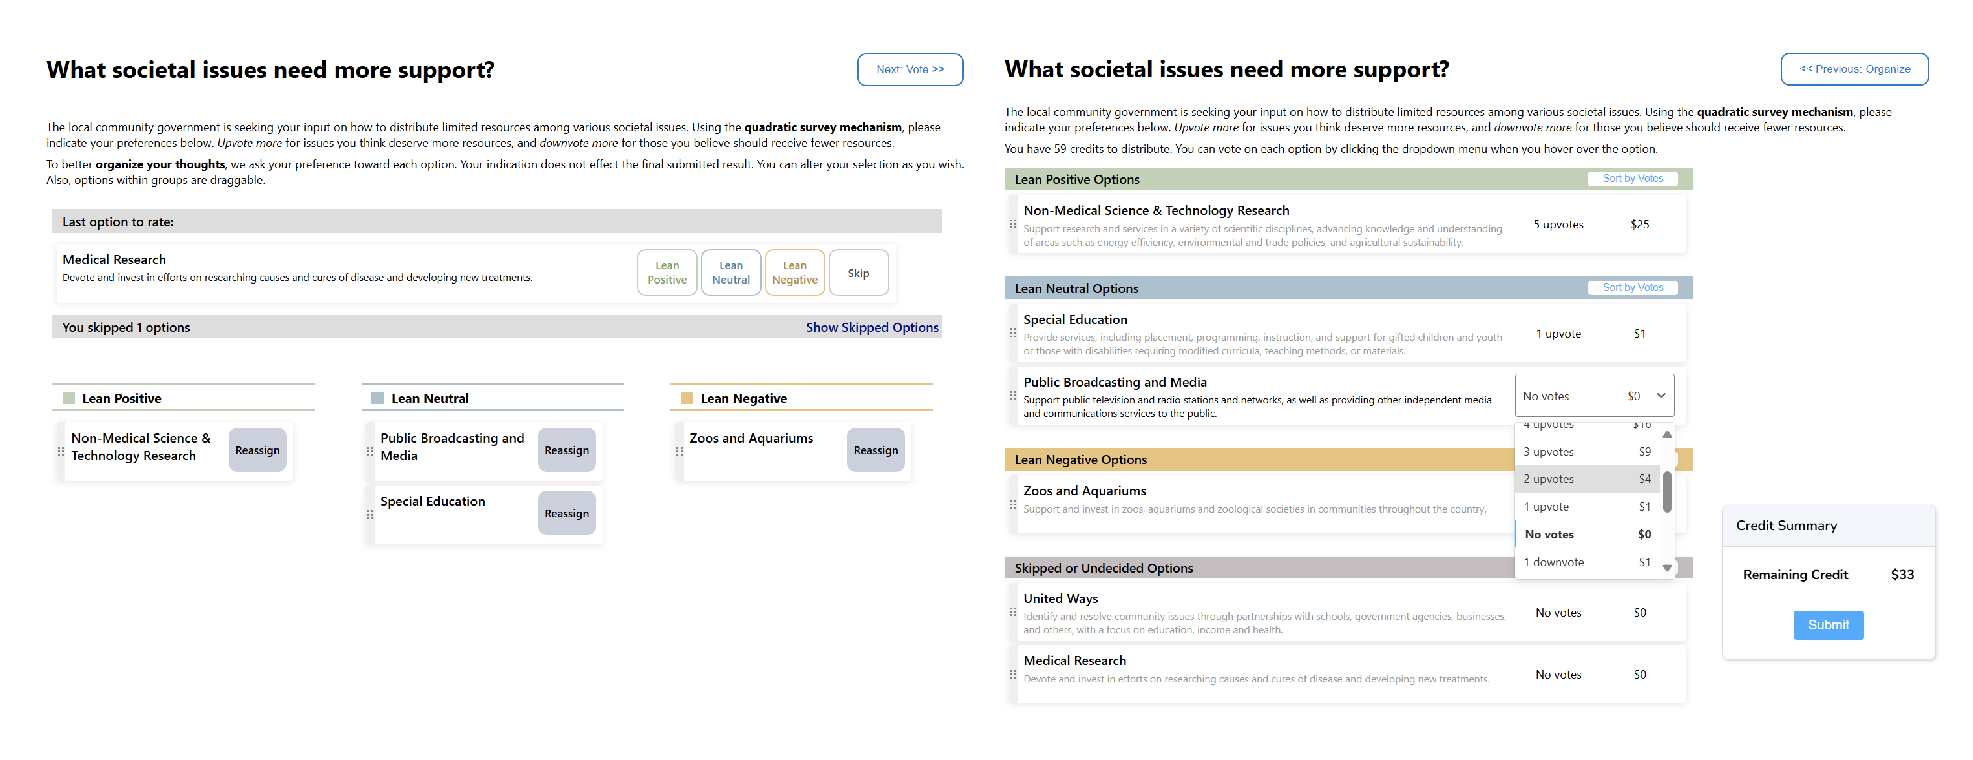
\includegraphics[width=\textwidth]{content/image/header.pdf}
%     \caption{A novel two-phase interactive interface for Quadratic Surveys detailed in Sec.~\ref{sec:finalInterfaceDesign}}
%     \label{fig:header}
% \end{figure}



% This challenge emphasizes the critical importance of designing and developing suitable interfaces for Quadratic Surveys to elicit truthful and in-depth preference information from respondents. Good design is essential; without it, the quality of collected data can suffer significantly. 
% These reasons strongly motivate  Addressing this question fills a important gap in the literature and enhances the practical utility of QS in capturing high-quality data across various applications.

% Highlight this is also the first work to investigate where people felt challenging when completing QS.
% At the same time, reducing cognitive load and making survey less challenging . Effective design may mitigate these overload challenges, ensuring that the Quadratic Survey mechanism fulfills its potential to capture detailed and accurate preferences. Thus, more concretely, this study focused on answering the following three research questions:

% 1. we design
% 2. we test across condition
% 3. understand what is difficult/hard through qualitative and quant responses
% --> design and usage recommendations

% Cited without details
% U.S. Colorado state government~\cite{rogersColoradoTriedNew2019}, the Democratic
%  Caucus of the House of Representatives~\cite{QuadraticVotingColorado} in the U.S., government-sponsored hackathons~\cite{teamTaiwanDigitalMinister}, and the recent Gov4git~\cite{Gov4gitDecentralizedPlatform2023}
% Despite the advocacy of Quadratic Voting by Posner and Weyl~\cite{posner2018radical}
% Political scientists have demonstrated that ballot designs alone can sway voter decisions~\cite{engstrom2020politics}, marketing and psychology researchers have examined how the presentation of questions influences responses~\cite{weijtersEffectRatingScale2010, kierujVariationsResponseStyle2010, toepoelSmileysStarsHearts2019}, and Human-Computer Interaction researchers have focused on evaluating and understanding web surveys and smart interfaces for surveys~\cite{farzandAestheticsEvaluatingResponse2024, xiaoTellMeYourself2020, pielotDidYouMisclick2024}. These studies highlight the importance of studying the interface and design for survey mechanisms.
% The Quadratic Mechanism is undeniably more complex than other voting and surveying mechanisms like the Likert scale survey~\cite{likertTechniqueMeasurementAttitudes1932}, where individuals select from a few responses, and Approval Voting~\cite{bramsApprovalVoting1978}, where participants mark as many options as they approve without constraints.

% Move this to related works.
% The effectiveness of eliciting these responses hinges upon the study protocol, survey mechanism, and design of the tool at hand~\cite{olsonWaysKnowingHCI2014, couperWebSurveyDesign2001, jackoHumancomputerInteractionHandbook2012}. While much research has explored the influence of the former two aspects, this research focuses on the design of a specific survey -- Quadratic Surveys. 

% Move this to discussion + contribution
% Thus, the primary goal of this study is to present a novel interactive interface designed for quadratic surveys, which could presumably extend to other applications that utilize the quadratic mechanism. 

% TODO, for a cleaner thesis statement in the first par? mention challenges and interface here before diving deeper.
% The importance of design in surveying tools, the growing usage of applications on the quadratic mechanism, and the lack of research on the design regarding quadratic mechanisms that one could apply, motivated our main research question: \textit{How can we design interactive interfaces to support participants in completing Quadratic Surveys?}

% Quadratic Surveys and other quadratic mechanism powered applications allow individuals 
% \begin{itemize}
% \item RQ1. How does the number of options on QS impact respondents' cognitive load?
% \item RQ2a. How does the interactive interface involving grouping and direct manipulation interface influence QS respondents' cognitive load compared to text-based interface?
% \item RQ2b. Across the two interfaces, what are the sources of cognitive load from?
% \item RQ3. What are differences in QS respondents' behaviors when coping with long lists of options?
% \end{itemize}

% Before answering these research questions, we iteratively designed and built an interactive interface informed by prior literature in the questionnaire and survey response format. Then, 